\section{Failure Analysis}
\label{sec:ch8-failure-analysis}

\phantomsection\label{rq:ch8-rq2-intro}
\begin{rqbox}[RQ2]
Does a probe on the coordinator's hidden states recover the correct sub-agent more accurately than classifiers trained on a fixed representation of the query text, such as raw word counts, TF-IDF weighting, or sentence embeddings?
\end{rqbox}


\noindent To answer \hyperref[rq:ch8-rq2-intro]{\textbf{RQ2}}, this section compares the probe with the three text-only classifiers on the \texttt{natural} and the \texttt{adversarial} tier. A request of the \texttt{natural} tier states a waived constraint, and the sub-agent that owns it is the decoy (Section~\ref{subsec:constraints-binding-waived}). The \texttt{adversarial} tier generates its requests in pairs: the two requests of a pair share most of their wording, and the correct sub-agent of each one is the decoy of the other (Section~\ref{subsec:difficulty-tiers}). The decoy and the pair are the cause of the lower accuracy of the text-only classifiers on these two tiers. The \texttt{plain} tier is deliberately excluded, because it introduces no difficulty and every text-only classifier scores close to ceiling accuracy on it.

The errors of the probe are first compared with the errors of each text-only classifier, to measure how much the two depend on each other. The probe, the coordinator and the text-only classifiers are then compared on how often each predicts the decoy, and on how often each predicts the same sub-agent for both requests of a pair. An advantage of the probe on these measures indicates that the binding constraint is encoded in the hidden states more accurately than in the representations of the request text that the text-only classifiers use.

\subsection{Error Dependence Across the Tiers}
\label{subsec:ch8-failure-dependence}

The errors of the probe are compared with the errors of the text-only classifiers to determine whether the hidden states encode information that the representations of the text-only classifiers do not encode. If the probe fails mostly on the same requests as a text-only classifier, its errors follow the text of the request as that classifier's errors do. If its errors are largely independent of the errors of the text-only classifiers, the hidden states are likely to encode information that these representations do not encode.

The coordinator is not included in this subsection because it is never trained on the requests of the dataset, unlike the probe and the text-only classifiers. The probe and the text-only classifiers are logistic regressions trained on the same labels and the same folds, and each receives a different input representation. A difference between their errors can therefore only come from this representation. A difference between the errors of the coordinator and the errors of a text-only classifier cannot be read the same way.

For each text-only classifier, the requests of a tier are divided into two groups: the requests where the text-only classifier is right and the requests where it is wrong. The following quantities are then computed for the probe, on each tier and against each text-only classifier:

\begin{itemize}
    \item \textbf{accuracy where the text-only classifier is right} ($a_p^{+}$): the accuracy of the probe on the requests where the text-only classifier is right;
    \item \textbf{accuracy where the text-only classifier is wrong} ($a_p^{-}$): the accuracy of the probe on the requests where the text-only classifier is wrong;
    \item \textbf{gap} ($g$): the difference $g = a_p^{-} - a_p^{+}$. A negative $g$ indicates that the probe is less accurate on the requests where the text-only classifier is wrong;
    \item \textbf{normalized kappa} ($\kappa_n$): measures how strongly the probe and the text-only classifier are right on the same requests and wrong on the same requests, on a scale from 0 for independent errors to 1 for the strongest agreement that the accuracies of the two allow.
\end{itemize}

The normalized kappa is derived from Cohen's kappa. For the probe and a text-only classifier, Cohen's kappa is computed as
\[
    \kappa = \frac{p_o - p_e}{1 - p_e},
\]
where:

\begin{itemize}
    \item $p_o$ is the fraction of requests on which the probe and the text-only classifier are both right or both wrong;
    \item $p_e$ is the value of $p_o$ expected from the accuracy of the probe and the accuracy of the text-only classifier if their errors were independent.
\end{itemize}

The highest value that $\kappa$ can reach depends on the accuracy $a_p$ of the probe and the accuracy $a_b$ of the text-only classifier. When the two accuracies differ, one of the two is right and the other is wrong on at least a fraction $|a_p - a_b|$ of the requests. Therefore $p_o$ is at most $1 - |a_p - a_b|$, and $\kappa$ is at most
\[
    \kappa_{\max} = \frac{1 - |a_p - a_b| - p_e}{1 - p_e}.
\]
The accuracies of the probe and of the text-only classifiers differ across text-only classifiers and tiers, so $\kappa_{\max}$ differs too, and the same value of $\kappa$ can indicate a weak agreement in one row of the comparison and a strong agreement in another. The normalized kappa removes this effect by dividing $\kappa$ by its highest reachable value:
\[
    \kappa_n = \frac{\kappa}{\kappa_{\max}}.
\]

If the errors of the probe do not depend on the errors of the text-only classifier, $g$ and $\kappa_n$ are close to 0 in absolute value. If the probe and the text-only classifier are right on the same requests and wrong on the same requests, $g$ is large and negative and $\kappa_n$ is close to 1. Table~\ref{tab:ch8-dependence} reports $a_p^{+}$, $a_p^{-}$, $g$ and $\kappa_n$ on the \texttt{natural} and \texttt{adversarial} tiers, and Figure~\ref{fig:ch8-dependence} plots $a_p^{+}$, $a_p^{-}$ and $g$.

In every row of Table~\ref{tab:ch8-dependence}, $a_p^{-}$ is lower than $a_p^{+}$, with $g$ between $-$0.028 and $-$0.179. Some of the requests on which the wording misleads the text-only classifiers therefore also mislead the probe. $\kappa_n$ between the probe and a text-only classifier is between 0.151 and 0.424. The absolute value of $g$ is larger on \texttt{adversarial} than on \texttt{natural} for every combination of dataset and text-only classifier. This shows that the difficulty of \texttt{adversarial} affects the probe more on the requests where a text-only classifier is wrong. Against the bag-of-words classifier, $\kappa_n$ is lower on \texttt{adversarial} than on \texttt{natural} on both datasets. Against the TF-IDF classifier, it is higher on the single-turn dataset and lower on the multi-turn dataset. Against the embedding classifier, it is higher on both datasets.

\begin{table}[H]
    \centering
    \small
    \begin{tabular}{@{}llcccc c cccc@{}}
        \toprule
        & & \multicolumn{4}{c}{\textbf{Single-turn}} & & \multicolumn{4}{c}{\textbf{Multi-turn}} \\
        \cmidrule(lr){3-6} \cmidrule(lr){8-11}
        \textbf{Tier} & \textbf{Classifier} & $\boldsymbol{a_p^{+}}$ & $\boldsymbol{a_p^{-}}$ & $\boldsymbol{g}$ & $\boldsymbol{\kappa_n}$ & & $\boldsymbol{a_p^{+}}$ & $\boldsymbol{a_p^{-}}$ & $\boldsymbol{g}$ & $\boldsymbol{\kappa_n}$ \\
        \midrule
        \texttt{natural}     & Bag-of-words & 0.958 & 0.878 & $-$0.080 & 0.356 & & \worst{0.944} & 0.891 & $-$0.053 & \worst{0.243} \\
                             & TF-IDF       & \best{0.959} & \worst{0.868} & \worst{$-$0.091} & \best{0.367} & & \best{0.950} & \worst{0.876} & \worst{$-$0.074} & \best{0.366} \\
                             & Embedding    & \worst{0.944} & \best{0.916} & \best{$-$0.028} & \worst{0.151} & & \worst{0.944} & \best{0.900} & \best{$-$0.044} & 0.268 \\
        \midrule
        \texttt{adversarial} & Bag-of-words & 0.888 & 0.749 & $-$0.139 & \worst{0.317} & & \worst{0.795} & 0.670 & \best{$-$0.125} & \worst{0.204} \\
                             & TF-IDF       & \best{0.905} & \worst{0.748} & \worst{$-$0.157} & \best{0.424} & & \best{0.833} & \worst{0.654} & \worst{$-$0.179} & \best{0.362} \\
                             & Embedding    & \worst{0.886} & \best{0.791} & \best{$-$0.095} & 0.321 & & 0.820 & \best{0.692} & $-$0.128 & 0.298 \\
        \bottomrule
    \end{tabular}
    \caption[Probe accuracy by classifier correctness, gap, and normalized kappa]{Accuracy of the probe on the requests where each text-only classifier is right ($a_p^{+}$) and on the requests where it is wrong ($a_p^{-}$), gap $g = a_p^{-} - a_p^{+}$, and normalized kappa $\kappa_n$ between the probe and the text-only classifier. Each value is the mean of the seven runs on the same dataset. In each tier and column, the highest value is in bold and the lowest is underlined.}
    \label{tab:ch8-dependence}
\end{table}

\begin{figure}[htbp]
    \centering
    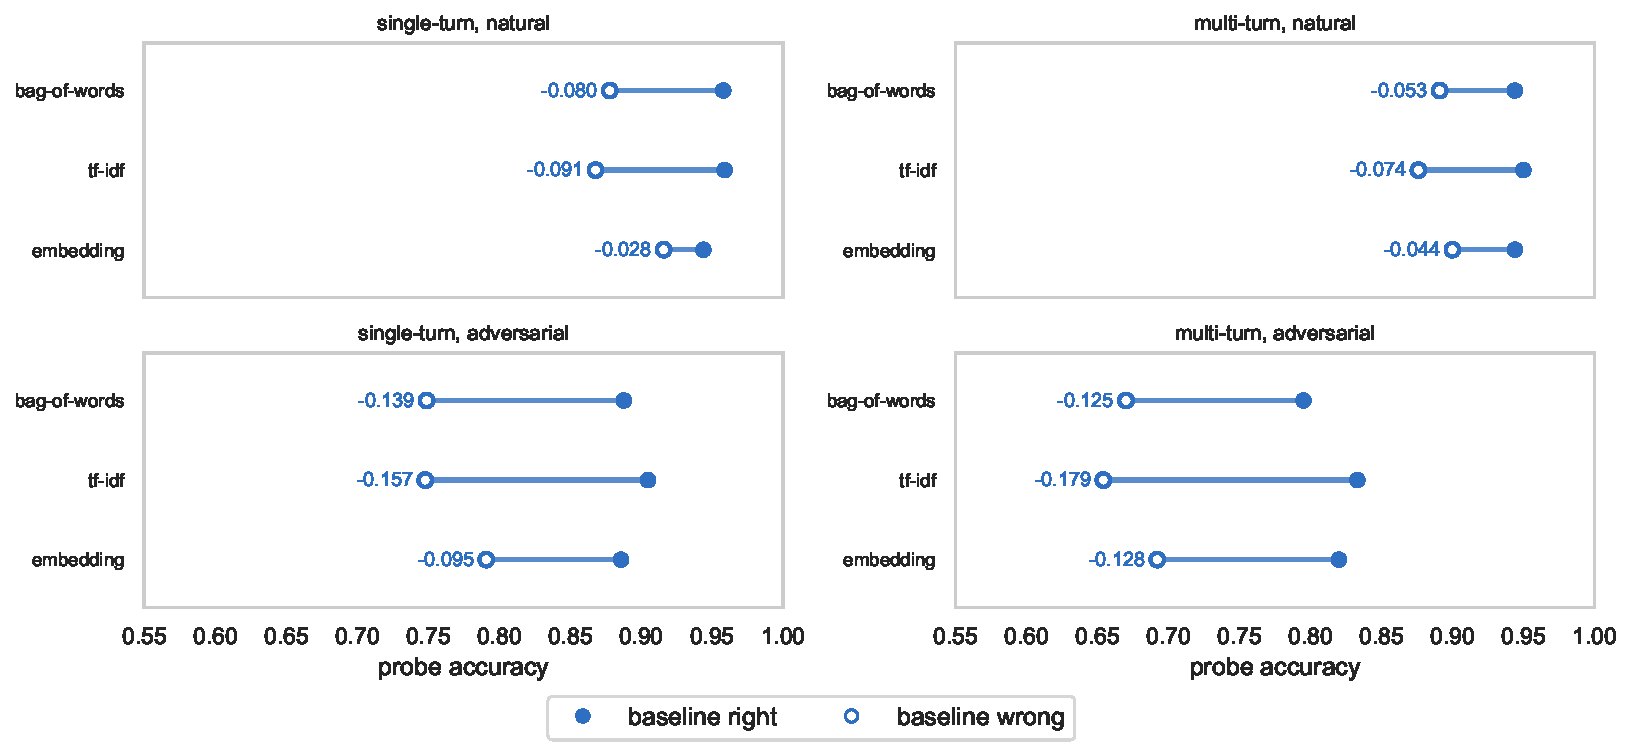
\includegraphics[width=\textwidth]{images/plots/overview/overview_dependence.pdf}
    \caption[Probe accuracy where each text-only classifier is right and where it is wrong]{Accuracy of the probe where each text-only classifier is right ($a_p^{+}$, filled end) and where it is wrong ($a_p^{-}$, hollow end), one panel per dataset and tier. The number at the hollow end is the gap $g$. Each value is the mean of the seven runs on the same dataset.}
    \label{fig:ch8-dependence}
\end{figure}

\FloatBarrier

\subsection{Adversarial Pairs}
\label{subsec:ch8-failure-pairs}

As described in Section~\ref{subsec:difficulty-tiers}, the \texttt{adversarial} tier of each dataset consists of 900 samples generated in 450 pairs. The two requests of a pair share most of their wording and differ only in the clause that names the constraint that is binding. Both requests state the same two constraints, and the constraint that is binding in one request is waived in the other, so the correct sub-agent of each request is the decoy of the other. The pairs are used to observe whether a classifier tells the two requests of a pair apart or predicts the same sub-agent for both, where a \emph{classifier} is any of the probe, the coordinator and the three text-only classifiers. Two quantities are computed for each classifier:

\begin{itemize}
    \item \textbf{both, one or neither right}: the share of pairs in which the classifier classifies both requests correctly, one of the two, or neither;
    \item \textbf{collapsed pairs}: the share of pairs in which the classifier predicts the same sub-agent for both requests. In a collapsed pair, at most one of the two requests is classified correctly.
\end{itemize}

Figure~\ref{fig:ch8-pairs} reports both quantities and shows that the probe is the only classifier that classifies both requests correctly in most pairs, on both datasets. The coordinator and the text-only classifiers classify only one of the two requests correctly in most pairs.

\begin{figure}[htbp]
    \centering
    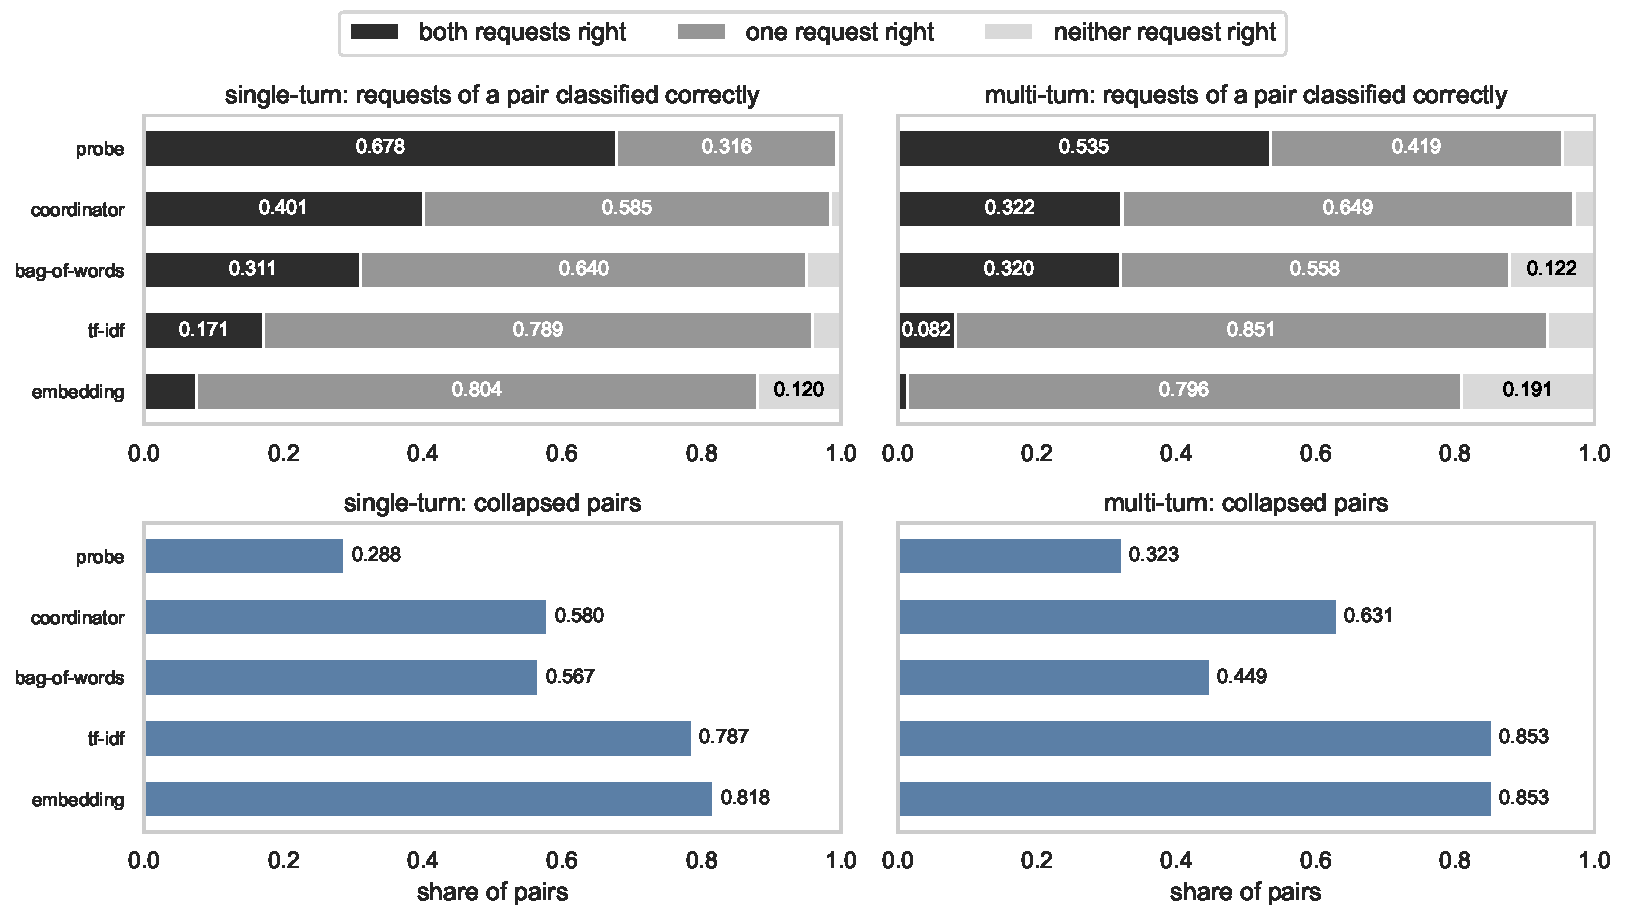
\includegraphics[width=\textwidth]{images/plots/overview/overview_pairs.pdf}
    \caption[Adversarial pair correctness and collapsed pairs per classifier]{Top: share of the 450 \texttt{adversarial} pairs in which each classifier classifies both, one or neither of the two requests correctly. Bottom: share of collapsed pairs. Single-turn dataset on the left, multi-turn dataset on the right. The probe and the coordinator values are the mean of the seven runs on the same dataset. The text-only classifiers do not depend on the model.}
    \label{fig:ch8-pairs}
\end{figure}

The probe collapses fewer pairs than the coordinator on both datasets, with a mean share of collapsed pairs of 0.288 and 0.323 against 0.580 and 0.631. The coordinator collapses fewer pairs than the TF-IDF and embedding classifiers, but more than the bag-of-words classifier, which has a share of collapsed pairs of 0.567 and 0.449. The probe also has the highest share of pairs with both requests right on both datasets, with a mean of 0.678 and 0.535 against 0.401 and 0.322 for the coordinator.

\FloatBarrier

\subsection{Decoy Predictions}
\label{subsec:ch8-failure-decoy}

On \texttt{natural} and \texttt{adversarial}, every request states a waived constraint, and the sub-agent that owns it is the decoy (Section~\ref{subsec:constraints-binding-waived}). The decoy predictions are used to observe how often each classifier is misled by the waived constraint, and whether the probe is misled less often than the coordinator and the text-only classifiers. The \emph{decoy rate} of a classifier is defined as the share of the samples of a tier on which the classifier predicts the decoy. Figure~\ref{fig:ch8-decoy} reports the decoy rate of every classifier.

\begin{figure}[htbp]
    \centering
    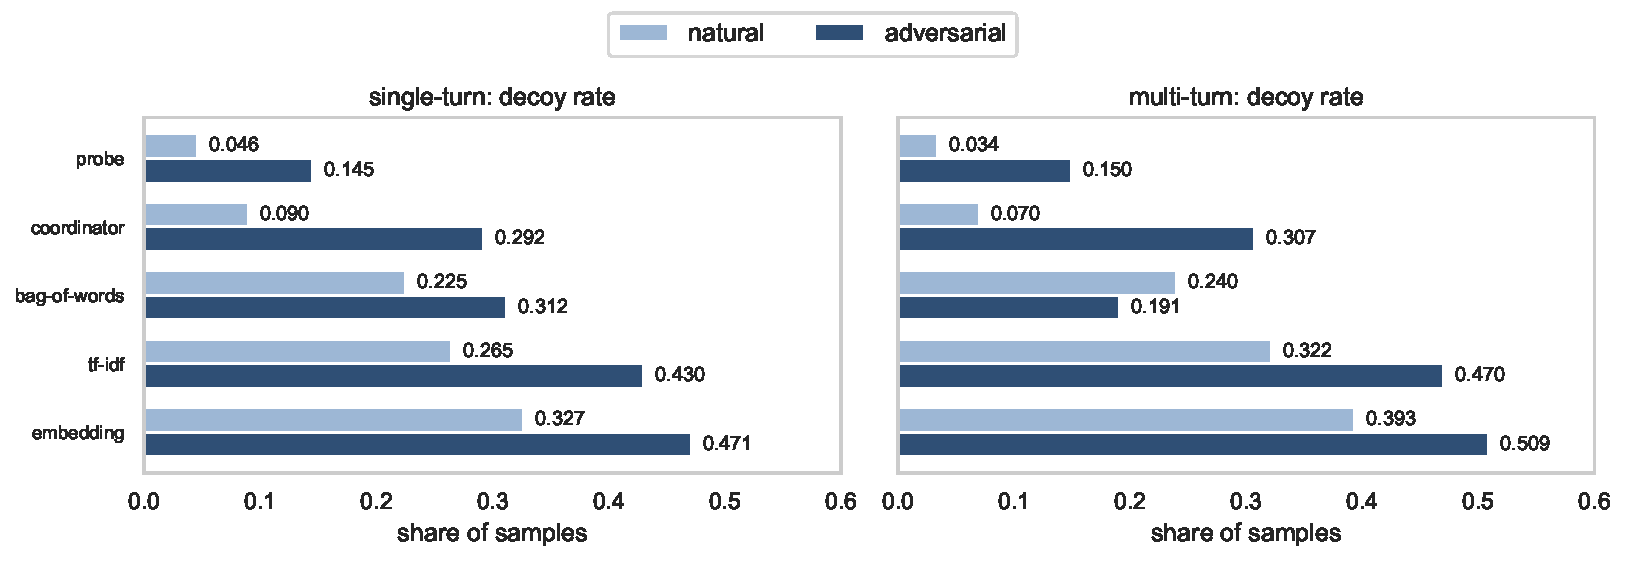
\includegraphics[width=\textwidth]{images/plots/overview/overview_decoy.pdf}
    \caption[Decoy rate by tier, single-turn and multi-turn datasets]{Decoy rate: share of the samples of each tier on which each classifier predicts the decoy, single-turn dataset on the left and multi-turn dataset on the right. The probe and the coordinator values are the mean of the seven runs on the same dataset. The text-only classifiers do not depend on the model.}
    \label{fig:ch8-decoy}
\end{figure}

The probe has the lowest mean decoy rate on both tiers and both datasets. The coordinator has the second lowest, except on the multi-turn \texttt{adversarial} tier, where the bag-of-words classifier has the second lowest.

The probe improves on the coordinator in the three measures of this section: on both datasets it has a lower mean share of collapsed pairs, a higher mean share of pairs with both requests right, and a lower mean decoy rate on both tiers. The correct sub-agent is therefore encoded in the hidden states of the coordinator, but the coordinator does not select it as accurately as the probe. This may come from the training of the probe, which learns to read the sub-agent from the hidden states on labeled samples of the dataset, while the coordinator chooses according to the routing policy stated in its prompt.

\subsection{Answer to RQ2}
\label{subsec:ch8-rq2-answer}

\phantomsection\label{rq:ch8-rq2}
\begin{rqbox}[RQ2]
Does a probe on the coordinator's hidden states recover the correct sub-agent more accurately than classifiers trained on a fixed representation of the query text, such as raw word counts, TF-IDF weighting, or sentence embeddings?
\end{rqbox}


\noindent Yes. Section~\ref{sec:ch7-observations} reports that the probe is more accurate than all three text-only classifiers on the \texttt{natural} and the \texttt{adversarial} tier of both datasets.

On the \texttt{adversarial} pairs, the probe has the lowest mean share of collapsed pairs and the highest mean share of pairs with both requests right on both datasets, and it has the lowest mean decoy rate on both tiers and both datasets. The binding constraint stated in a request can therefore be read more accurately from the hidden state at the last prompt token than from the representations of the request text that the text-only classifiers use.

The advantage is partial, because the errors of the probe partly follow the errors of the text-only classifiers: $a_p^{-}$ is lower than $a_p^{+}$ in every comparison of Table~\ref{tab:ch8-dependence}, with $\kappa_n$ between 0.151 and 0.424.

\FloatBarrier
